\subsection{假设检验}\label{sec:10.3}
与\autoref{sec:10.1}一样，本节介绍几种在复杂问题中导出某些检验的方法. 所考虑的问题，是先前定义的最优检验不存在（例如不存在UMP无偏检验），或尚不知道最优检验的问题. 此时，导出任何合理的检验都可能有用. 以下两小节讨论似然比检验的大样本性质，以及其他近似大样本检验.

\subsubsection{似然比检验的渐近分布}\label{sec:10.3.1}
对复杂模型，构造检验最有用的方法之一是似然比法，因为它明确地定义检验统计量
$$\lambda(\boldsymbol x)=\frac{\sup_{\Theta_0}L(\theta\mid\boldsymbol x)}{\sup_\Theta L(\theta\mid\boldsymbol x)},$$
并明确给出拒绝域的形式$\{\boldsymbol x:\lambda(\boldsymbol x)\leq c\}$. 观测到数据$\boldsymbol X=\boldsymbol x$后，似然函数$L(\theta\mid\boldsymbol x)$就是变量$\theta$的完全确定的函数.
\sourcepageanchor{426}
即使不能解析地求出$L(\theta\mid\boldsymbol x)$在$\Theta_0$和$\Theta$上的两个上确界，通常也能数值计算. 因此，即使没有定义$\lambda(\boldsymbol x)$的方便公式，也能对观测数据点求得检验统计量$\lambda(\boldsymbol x)$.

为定义水平$\alpha$的检验，必须选择常数$c$使
\begin{equation}\label{eq:10.3.1}
\sup_{\theta\in\Theta_0}P_\theta\bigl(\lambda(\boldsymbol X)\leq c\bigr)\leq\alpha.
\end{equation}
若不能导出$\lambda(\boldsymbol x)$的简单公式，似乎就无望求出$\lambda(\boldsymbol X)$的抽样分布，从而知道如何选$c$以保证\eqref{eq:10.3.1}. 但借助渐近理论，可以获得近似答案.

类似\autoref{thm:10.1.12}，有如下结果.

\begin{theorem}[LRT的渐近分布：简单$H_0$]\label{thm:10.3.1}
为检验$H_0:\theta=\theta_0$对$H_1:\theta\ne\theta_0$，假设$X_1,\ldots,X_n$独立同分布于$f(x\mid\theta)$，$\hat\theta$为$\theta$的MLE，且$f(x\mid\theta)$满足\hyperref[sec:10.6.2]{杂录10.6.2}中的正则条件. 则在$H_0$下，当$n\to\infty$时，
$$-2\log\lambda(\boldsymbol X)\longrightarrow\chi_1^2\quad\text{依分布},$$
其中$\chi_1^2$是自由度为1的卡方随机变量.
\end{theorem}
\begin{proof}
首先在$\hat\theta$处对$\log L(\theta\mid\boldsymbol x)=l(\theta\mid\boldsymbol x)$作泰勒展开，得到
$$l(\theta\mid\boldsymbol x)=l(\hat\theta\mid\boldsymbol x)+l'(\hat\theta\mid\boldsymbol x)(\theta-\hat\theta)+l''(\hat\theta\mid\boldsymbol x)\frac{(\theta-\hat\theta)^2}{2!}+\cdots.$$
现将$l(\theta_0\mid\boldsymbol x)$的展开式代入$-2\log\lambda\boldsymbol x=-2l(\theta_0\mid\boldsymbol x)+2l(\hat\theta\mid\boldsymbol x)$，得到\footnote{译注：原文下式把平方差除以$-l''$；由上面的泰勒展开应为$-l''(\hat\theta\mid\boldsymbol x)(\theta_0-\hat\theta)^2$，或除以观测信息量的倒数. 分子原文还写$\theta$而非$\theta_0$. 原式及随后“分母”一词保留.}
$$-2\log\lambda(\boldsymbol x)\approx\frac{(\theta-\hat\theta)^2}{-l''(\hat\theta\mid\boldsymbol x)},$$
其中使用$l'(\hat\theta\mid\boldsymbol x)=0$. 由于分母是观测信息量$\hat I_n(\hat\theta)$，且$\frac1n\hat I_n(\hat\theta)\to I(\theta_0)$，由\autoref{thm:10.1.12}和Slutsky定理（\autoref{thm:5.5.17}），得到$-2\log\lambda(\boldsymbol X)\to\chi_1^2$.
\end{proof}

\begin{example}[泊松LRT]\label{ex:10.3.2}
基于独立同分布于Poisson$(\lambda)$的观测$X_1,\ldots,X_n$，检验$H_0:\lambda=\lambda_0$对$H_1:\lambda\ne\lambda_0$，有
$$-2\log\lambda(\boldsymbol X)=-2\log\left(\frac{e^{-n\lambda_0}\lambda_0^{\sum x_i}}{e^{-n\hat\lambda}\hat\lambda^{\sum x_i}}\right)
=2n\bigl[(\lambda_0-\hat\lambda)-\hat\lambda\log(\lambda_0/\hat\lambda)\bigr],$$
其中$\hat\lambda=\sum x_i/n$是$\lambda$的MLE. 应用\autoref{thm:10.3.1}，当$-2\log\lambda(\boldsymbol x)>\chi_{1,\alpha}^2$时，在水平$\alpha$下拒绝$H_0$.

为了解渐近近似的准确程度，对检验统计量作一个小型模拟. 取$\lambda_0=5$、$n=25$，\autoref{fig:10.3.1}画出$-2\log\lambda(\boldsymbol x)$的10,000个值的直方图，以及$\chi_1^2$的pdf. 二者吻合似乎相当合理. 此外，\autoref{tab:10.3.5}比较模拟（精确）临界点与$\chi_1^2$（近似）临界点，显示它们非常接近.
\end{example}

\autoref{thm:10.3.1}可推广到原假设涉及参数向量的情形. 下面的推广不予证明，它至少对大样本保证\eqref{eq:10.3.1}成立. 完整讨论见\hyperref[bib:source311]{Stuart、Ord和Arnold（1999}，第22章）.

\sourcepageanchor{427}
\par\begin{figure}[htbp]\centering
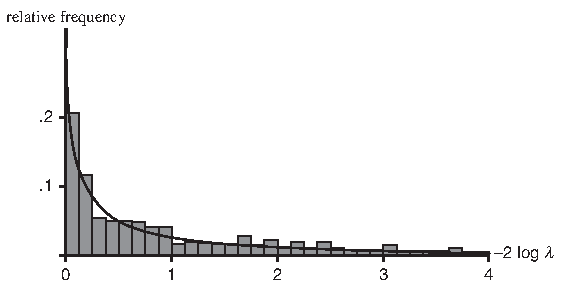
\includegraphics[width=.73\textwidth]{assets/chapter10/fig-10.3.1.pdf}
\caption{$-2\log\lambda(\boldsymbol x)$的10,000个值的直方图，以及$\chi_1^2$的pdf；$\lambda_0=5$，$n=25$.}\label{fig:10.3.1}
\end{figure}\par
\par\begin{table}[htbp]\centering\setcounter{table}{4}
\caption{泊松LRT统计量的模拟（精确）百分位数与近似百分位数}\label{tab:10.3.5}
\begin{tabular}{lrrrr}\toprule
百分位&.80&.90&.95&.99\\\midrule
模拟&1.630&2.726&3.744&6.304\\
$\chi^2$&1.642&2.706&3.841&6.635\\\bottomrule
\end{tabular}
\end{table}\par

\begin{theorem}\label{thm:10.3.3}\index{SI0632@渐近}
设$X_1,\ldots,X_n$是来自pdf或pmf $f(x\mid\theta)$的随机样本. 在\hyperref[sec:10.6.2]{杂录10.6.2}的正则条件下，若$\theta\in\Theta_0$，则统计量$-2\log\lambda(\boldsymbol X)$的分布随着样本量$n\to\infty$收敛到卡方分布. 极限分布的自由度，是$\theta\in\Theta_0$所规定的自由参数个数与$\theta\in\Theta$所规定的自由参数个数之差.
\end{theorem}

当$\lambda(\boldsymbol X)$较小时拒绝$H_0:\theta\in\Theta_0$，等价于当$-2\log\lambda(\boldsymbol X)$较大时拒绝. 因此，
$$\text{拒绝$H_0$当且仅当}\quad-2\log\lambda(\boldsymbol X)\geq\chi_{\nu,\alpha}^2,$$
其中$\nu$为\autoref{thm:10.3.3}规定的自由度. 若$\theta\in\Theta_0$且样本量大，第一类错误概率近似为$\alpha$.\index{SI0509@渐近}\semanticindexanchor{509:427} 这样，样本量大时\eqref{eq:10.3.1}近似满足，便定义了渐近大小为$\alpha$的检验. 注意，定理实际上仅意味着
$$\lim_{n\to\infty}P_\theta(\text{拒绝$H_0$})=\alpha\quad\text{对每个$\theta\in\Theta_0$},$$
并不意味着$\sup_{\theta\in\Theta_0}P_\theta(\text{拒绝$H_0$})$收敛到$\alpha$. 渐近大小为$\alpha$的检验通常如此.

检验统计量自由度的计算通常很直接. 最常见的是，$\Theta$可表示为$q$维欧氏空间的子集，并包含$\mathbb R^q$中的一个开子集；$\Theta_0$可表示为$p$维欧氏空间的子集，并包含$\mathbb R^p$中的一个开子集，其中$p<q$. 则$q-p=\nu$是检验统计量的自由度.

\begin{example}[多项LRT]\label{ex:10.3.4}\index{SI0636@多项}
设$\theta=(p_1,p_2,p_3,p_4,p_5)$，其中$p_j$非负且和为1. 假设$X_1,\ldots,X_n$为独立同分布的离散随机变量，$P_\theta(X_i=j)=p_j$，$j=1,\ldots,5$. 因此$X_i$的pmf为$f(j\mid\theta)=p_j$，似然函数为
$$L(\theta\mid\boldsymbol x)=\prod_{i=1}^nf(x_i\mid\theta)=p_1^{y_1}p_2^{y_2}p_3^{y_3}p_4^{y_4}p_5^{y_5},$$
\sourcepageanchor{428}
其中$y_j$为$x_1,\ldots,x_n$中等于$j$的个数. 考虑检验
$$H_0:p_1=p_2=p_3\text{且}p_4=p_5\qquad\text{对}\qquad H_1:H_0\text{不成立}.$$
完整参数空间$\Theta$实际上是四维集合. 因为$p_5=1-p_1-p_2-p_3-p_4$，只有四个自由参数. 参数集合由
$$\sum_{j=1}^4p_j\leq1\quad\text{且}\quad p_j\geq0,\quad j=1,\ldots,4$$
定义，是包含$\mathbb R^4$中开子集的$\mathbb R^4$子集. 因此$q=4$. $H_0$规定的集合只有一个自由参数，因为一旦固定$p_1$，$0\leq p_1\leq1/3$，则$p_2=p_3$必须等于$p_1$，而$p_4=p_5$必须等于$(1-3p_1)/2$. 因而$p=1$，自由度$\nu=4-1=3$.

计算$\lambda(\boldsymbol x)$，必须确定$\theta$在$\Theta_0$和$\Theta$下的MLE. 令
$$\frac\partial{\partial p_j}\log L(\theta\mid\boldsymbol x)=0\quad\text{对每个$j=1,\ldots,4$},$$
并利用$p_5=1-p_1-p_2-p_3-p_4$及$y_5=n-y_1-y_2-y_3-y_4$，可验证$p_j$在$\Theta$下的MLE为$\hat p_j=y_j/n$. 在$H_0$下，似然函数化为
$$L(\theta\mid\boldsymbol x)=p_1^{y_1+y_2+y_3}\left(\frac{1-3p_1}2\right)^{y_4+y_5}.$$
同样，以令导数为零的通常方法可得，$H_0$下$p_1$的MLE为$\hat p_{10}=(y_1+y_2+y_3)/(3n)$. 此时$\hat p_{10}=\hat p_{20}=\hat p_{30}$，且$\hat p_{40}=\hat p_{50}=(1-3\hat p_{10})/2$. 将这些值和$\hat p_j$代入$L(\theta\mid\boldsymbol x)$，合并相同指数的项，得到
$$\begin{aligned}
\lambda(\boldsymbol x)&=\left(\frac{y_1+y_2+y_3}{3y_1}\right)^{y_1}\left(\frac{y_1+y_2+y_3}{3y_2}\right)^{y_2}\left(\frac{y_1+y_2+y_3}{3y_3}\right)^{y_3}\\
&\quad\times\left(\frac{y_4+y_5}{2y_4}\right)^{y_4}\left(\frac{y_4+y_5}{2y_5}\right)^{y_5}.
\end{aligned}$$
因此检验统计量为
\begin{equation}\label{eq:10.3.2}
-2\log\lambda(\boldsymbol x)=2\sum_{i=1}^5y_i\log\left(\frac{y_i}{m_i}\right),
\end{equation}
其中$m_1=m_2=m_3=(y_1+y_2+y_3)/3$，$m_4=m_5=(y_4+y_5)/2$. 渐近大小为$\alpha$的检验在$-2\log\lambda(\boldsymbol x)\geq\chi_{3,\alpha}^2$时拒绝$H_0$. 本例属于广泛使用似然比检验渐近理论的一大类检验问题.
\end{example}

\subsubsection{其他大样本检验}\label{sec:10.3.2}\index{SI0204@依分布}
构造大样本检验统计量的另一常用方法，基于具有渐近正态分布的估计量. 假设要检验关于实值参数$\theta$的假设，$W_n=W(X_1,\ldots,X_n)$是通过某种方法导出的、基于容量$n$样本的$\theta$的点估计量. 例如，$W_n$可以是$\theta$的MLE. 基于正态近似的近似检验，可按如下方式论证. 若$\sigma_n^2$表示$W_n$的方差，且能用某种形式的中心极限定理证明，当$n\to\infty$时，$(W_n-\theta)/\sigma_n$依分布收敛到标准正态随机变量，那么就可以将$(W_n-\theta)/\sigma_n$与$\mathrm n(0,1)$分布比较，由此得到近似检验的基础.

当然，上段论证有许多细节需要验证，但这一思想确实适用于许多情形. 例如，若$W_n$为MLE，可以用\autoref{thm:10.1.12}来确立上述论证. 注意，$W_n$的分布以及可能的$\sigma_n$值依赖于$\theta$. 因而，更正式地说，对每个固定的$\theta\in\Theta$，若采用$W_n$相应的分布和$\sigma_n$相应的值，则$(W_n-\theta)/\sigma_n$收敛到标准正态分布.
\sourcepageanchor{429}
若对每个$n$，$\sigma_n$是可计算的常数（可依赖$\theta$，但不依赖其他未知参数），便可能导出基于$(W_n-\theta)/\sigma_n$的检验.

在一些情形中，$\sigma_n$还依赖未知参数.\index{SI0979@Slutsky定理}\semanticindexanchor{979:429} 此时寻找$\sigma_n$的估计$S_n$，使$\sigma_n/S_n$依概率收敛到1. 再由Slutsky定理（像\autoref{ex:5.5.18}一样），推出$(W_n-\theta)/S_n$也依分布收敛到标准正态分布. 大样本检验可据此构造.

假设要检验双侧假设$H_0:\theta=\theta_0$对$H_1:\theta\ne\theta_0$. 近似检验可基于统计量$Z_n=(W_n-\theta_0)/S_n$，当且仅当$Z_n<-z_{\alpha/2}$或$Z_n>z_{\alpha/2}$时拒绝$H_0$. 若$H_0$成立，则$\theta=\theta_0$，$Z_n$依分布收敛到$Z\sim\mathrm n(0,1)$. 因此，第一类错误概率
$$P_{\theta_0}(Z_n<-z_{\alpha/2}\text{或}Z_n>z_{\alpha/2})\longrightarrow P(Z<-z_{\alpha/2}\text{或}Z>z_{\alpha/2})=\alpha,$$
所以它是渐近大小为$\alpha$的检验.

现考虑备择参数值$\theta\ne\theta_0$. 可写为
\begin{equation}\label{eq:10.3.3}
Z_n=\frac{W_n-\theta_0}{S_n}=\frac{W_n-\theta}{S_n}+\frac{\theta-\theta_0}{S_n}.
\end{equation}
无论$\theta$取何值，都有$(W_n-\theta)/S_n\to\mathrm n(0,1)$. 通常还满足$n\to\infty$时$\sigma_n\to0$. （回顾$\sigma_n=\operatorname{Var}W_n$，而估计量通常随着$n\to\infty$越来越精确.）\footnote{译注：原文括号内写$\sigma_n=\operatorname{Var}W_n$，与前文$\sigma_n^2$为方差的定义不符；应为$\sigma_n^2=\operatorname{Var}W_n$. 原文保留.} 因而$S_n$依概率收敛到0，$(\theta-\theta_0)/S_n$根据$\theta-\theta_0$为正或负，分别依概率收敛到$+\infty$或$-\infty$. 于是$Z_n$也依概率收敛到$+\infty$或$-\infty$，且
$$P_\theta(\text{拒绝$H_0$})=P_\theta(Z_n<-z_{\alpha/2}\text{或}Z_n>z_{\alpha/2})\longrightarrow1,\qquad n\to\infty.$$
这样就能构造渐近大小为$\alpha$、渐近功效为1的检验.

若要检验单侧假设$H_0:\theta\leq\theta_0$对$H_1:\theta>\theta_0$，也能构造类似检验. 仍使用统计量$Z_n=(W_n-\theta_0)/S_n$，当且仅当$Z_n>z_\alpha$时拒绝$H_0$. 与上面类似的推理表明，检验的功效函数在$\theta<\theta_0$、$\theta=\theta_0$、$\theta>\theta_0$时分别收敛到0、$\alpha$、1. 所以该检验也有合理的渐近功效性质.

一般地，Wald检验（Wald test）是基于如下形式统计量的检验：
$$Z_n=\frac{W_n-\theta_0}{S_n},$$
其中$\theta_0$是参数$\theta$的假设值，$W_n$是$\theta$的估计量，$S_n$是$W_n$的标准误，即$W_n$标准差的估计. 若$W_n$是$\theta$的MLE，则如\autoref{sec:10.1.3}所述，$1/\sqrt{I(W_n)}$是合理的标准误. 也常使用$1/\sqrt{\hat I(W_n)}$，其中
$$\hat I(W_n)=-\left.\frac{\partial^2}{\partial\theta^2}\log L(\theta\mid\boldsymbol X)\right|_{\theta=W_n}$$
是观测信息量（见\eqref{eq:10.1.7}）.

\begin{example}[大样本二项检验]\label{ex:10.3.5}\index{SI0486@伯努利}
设$X_1,\ldots,X_n$为Bernoulli$(p)$总体的随机样本. 考虑检验$H_0:p\leq p_0$对$H_1:p>p_0$，其中$0<p_0<1$为指定值. 容量$n$样本中$p$的MLE为$\hat p_n=\sum_{i=1}^nX_i/n$. 因为$\hat p_n$就是样本均值，中心极限定理适用，且说明对任意$0<p<1$，$(\hat p_n-p)/\sigma_n$收敛到标准正态随机变量. 这里$\sigma_n=\sqrt{p(1-p)/n}$，依赖未知参数$p$.
\sourcepageanchor{430}
$\sigma_n$的合理估计为$S_n=\sqrt{\hat p_n(1-\hat p_n)/n}$，而且可以证明（\autoref{exercise:5.32}）$\sigma_n/S_n$依概率收敛到1. 因而，对任意$0<p<1$，
$$\frac{\hat p_n-p}{\sqrt{\hat p_n(1-\hat p_n)/n}}\longrightarrow\mathrm n(0,1).$$
将$p$替换为$p_0$，即定义了Wald检验统计量$Z_n$；大样本Wald检验在$Z_n>z_\alpha$时拒绝$H_0$. 作为$\sigma_n$的另一种估计，容易验证$1/I(\hat p_n)=\hat p_n(1-\hat p_n)/n$. 所以用信息量导出$\hat p_n$的标准误，也得到相同统计量$Z_n$.

若要检验双侧假设$H_0:p=p_0$对$H_1:p\ne p_0$，其中$0<p_0<1$为指定值，上述策略仍适用. 但此时还有另一种近似检验. 由中心极限定理，对任意$0<p<1$，
$$\frac{\hat p_n-p}{\sqrt{p(1-p)/n}}\longrightarrow\mathrm n(0,1).$$
因此，若原假设成立，统计量
\begin{equation}\label{eq:10.3.4}
Z'_n=\frac{\hat p_n-p_0}{\sqrt{p_0(1-p_0)/n}}\sim\mathrm n(0,1)\qquad\text{（近似地）}.
\end{equation}
近似水平$\alpha$的检验在$|Z'_n|>z_{\alpha/2}$时拒绝$H_0$.

当两个检验均适用时，例如检验$H_0:p=p_0$时，并不清楚应优先选择哪个. 它们的（实际而非近似）功效函数彼此交叉，所以每个检验都在参数空间的某一部分更有功效. （\hyperref[bib:source139]{Ghosh，1979}，对这个问题提供了一些见解. \hyperref[bib:source254]{Robbins，1977}，以及\hyperref[bib:source105]{Eberhardt和Fligner，1977}，讨论了相关的双样本二项问题争论. \autoref{exercise:10.31}给出该问题的两个不同检验统计量.）

当然，比较功效函数时会受到一个事实的干扰：这些是近似检验，不一定保持水平$\alpha$. 连续性校正（\autoref{ex:3.3.2}）有助于解决这个问题. 许多情形下，使用连续性校正的近似程序是保守的，即保持其名义$\alpha$水平（见\autoref{ex:10.4.6}）.
\end{example}

\eqref{eq:10.3.4}是另一种有用的大样本检验——得分检验（score test）——的特例. 定义得分统计量为
$$S(\theta)=\frac\partial{\partial\theta}\log f(\boldsymbol X\mid\theta)=\frac\partial{\partial\theta}\log L(\theta\mid\boldsymbol X).$$
由\eqref{eq:7.3.8}，对所有$\theta$，$E_\theta S(\theta)=0$. 特别地，若检验$H_0:\theta=\theta_0$且$H_0$成立，则$S(\theta_0)$均值为零. 此外，由\eqref{eq:7.3.10}，
$$\operatorname{Var}_\theta S(\theta)=E_\theta\left(\left(\frac\partial{\partial\theta}\log L(\theta\mid\boldsymbol X)\right)^2\right)
=-E_\theta\left(\frac{\partial^2}{\partial\theta^2}\log L(\theta\mid\boldsymbol X)\right)=I(\theta);$$
信息量就是得分统计量的方差. 得分检验的检验统计量为
$$Z_S=S(\theta_0)/\sqrt{I(\theta_0)}.$$
若$H_0$成立，$Z_S$均值为0、方差为1. 由\autoref{thm:10.1.12}，在$H_0$成立时，$Z_S$收敛到标准正态随机变量. 因此，近似水平$\alpha$的得分检验在$|Z_S|>z_{\alpha/2}$时拒绝$H_0$. 若$H_0$为复合假设，则在$Z_S$中用假定$H_0$成立时$\theta$的估计$\hat\theta_0$替代$\theta_0$. 若$\hat\theta_0$是受限MLE，受限极大化可借助拉格朗日乘子完成. 因而得分检验有时称为拉格朗日乘子检验（Lagrange multiplier test）.

\sourcepageanchor{431}
\begin{example}[二项得分检验]\label{ex:10.3.6}
再次考虑\autoref{ex:10.3.5}的伯努利模型，检验$H_0:p=p_0$对$H_1:p\ne p_0$. 直接计算得到
$$S(p)=\frac{\hat p_n-p}{p(1-p)/n}\quad\text{且}\quad I(p)=\frac n{p(1-p)}.$$
所以得分统计量为
$$Z_S=\frac{S(p_0)}{\sqrt{I(p_0)}}=\frac{\hat p_n-p_0}{\sqrt{p_0(1-p_0)/n}},$$
与\eqref{eq:10.3.4}相同.
\end{example}

最后考虑的一类近似检验是稳健检验（robust tests，见\hyperref[sec:10.6.6]{杂录10.6.6}）. 在\autoref{sec:10.2}看到，若$X_1,X_2,\ldots,X_n$是来自位置族的独立同分布样本，$\hat\theta_M$为$M$估计量，则
\begin{equation}\label{eq:10.3.5}
\sqrt n(\hat\theta_M-\theta_0)\longrightarrow\mathrm n\bigl(0,\operatorname{Var}_{\theta_0}(\hat\theta_M)\bigr),
\end{equation}
其中$\operatorname{Var}_{\theta_0}(\hat\theta_M)=E_{\theta_0}\psi(X-\theta_0)^2/[E_{\theta_0}\psi'(X-\theta_0)]^2$为渐近方差. 因此，可以构造“广义”得分统计量
$$Z_{GS}=\sqrt n\frac{\hat\theta_M-\theta_0}{\sqrt{\operatorname{Var}_{\theta_0}(\hat\theta_M)}},$$
或广义Wald统计量
$$Z_{GW}=\sqrt n\frac{\hat\theta_M-\theta_0}{\sqrt{\widehat{\operatorname{Var}}_{\theta_0}(\hat\theta_M)}},$$
其中$\widehat{\operatorname{Var}}_{\theta_0}(\hat\theta_M)$可为任意相合估计量. 例如，可以使用标准误的自助法估计，或直接将估计量代入\eqref{eq:10.2.6}而使用
\begin{equation}\label{eq:10.3.6}
\widehat{\operatorname{Var}}_1(\hat\theta_M)=\frac{\frac1n\sum_{i=1}^n[\psi(x_i-\hat\theta_M)]^2}{\left[\frac1n\sum_{i=1}^n\psi'(x_i-\hat\theta_M)\right]^2}.
\end{equation}
方差估计的选择可能很重要；相关指导见\hyperref[bib:source41]{Boos（1992）}或\hyperref[bib:source62]{Carroll等（1995}，附录A.3）.

\begin{example}[基于Huber估计量的检验]\label{ex:10.3.7}
若$X_1,X_2,\ldots,X_n$独立同分布于pdf $f(x-\theta)$，其中$f$关于零对称，则采用\eqref{eq:10.2.2}的$\rho$函数和\eqref{eq:10.2.7}的$\psi$函数的Huber $M$估计量，其渐近方差为
\begin{equation}\label{eq:10.3.7}
\frac{\int_{-k}^kx^2f(x)\,dx+k^2P_0(|X|>k)}{[P_0(|X|\leq k)]^2}.
\end{equation}
因此，根据$M$估计量的渐近正态性，例如可以在$|Z_{GS}|>z_{\alpha/2}$时拒绝$H_0$，以水平$\alpha$检验$H_0:\theta=\theta_0$对$H_1:\theta\ne\theta_0$. 为更切合实际，考察使用估计标准误的近似检验. 采用统计量$Z_{GW}$，但以\eqref{eq:10.3.7}为方差估计的基础，即\footnote{译注：下面分母原文为“1减去区间内比例”的平方；由\eqref{eq:10.3.7}应是区间内比例本身的平方，或将指标改为区间外. 原式保留.}
\begin{equation}\label{eq:10.3.8}
\widehat{\operatorname{Var}}_2(\hat\theta_M)=
\frac{\frac1n\sum_{i=1}^n(x_i-\hat\theta_M)^2I(|x_i-\hat\theta_M|<k)+k^2\left(\frac1n\sum_{i=1}^nI(|x_i-\hat\theta_M|>k)\right)}{\left(1-\frac1n\sum_{i=1}^nI(|x_i-\hat\theta_M|<k)\right)^2}.
\end{equation}
\sourcepageanchor{432}
另外加入一个“朴素”检验$Z_N$，使用简单的方差估计
\begin{equation}\label{eq:10.3.9}
\widehat{\operatorname{Var}}_3(\hat\theta_M)=\frac1n\sum_{i=1}^n(x_i-\hat\theta_M)^2.
\end{equation}
这些检验表现如何？解析评价很困难，但下面的小型模拟显示，$z_{\alpha/2}$临界值通常太小（忽略了方差估计的变动），实际大小一般大于名义大小. 不过，在一系列分布中的表现相当一致，双指数分布的情形最好. （最后这一点并不十分意外，因为Huber估计量对具有指数尾的分布享有一种最优性性质，见\hyperref[bib:source171]{Huber，1981}，第4章.）
\end{example}

\par\begin{table}[htbp]\centering
\caption{指定参数值处，基于$Z_{GW}$与$Z_N$的名义$\alpha=.1$检验的功效；样本量$n=15$，10,000次模拟.}\label{tab:10.3.6}
\small\begin{tabular}{lrrrrrrrr}\toprule
&\multicolumn{8}{c}{基础pdf}\\\cmidrule(lr){2-9}
&\multicolumn{2}{c}{正态}&\multicolumn{2}{c}{$t_5$}&\multicolumn{2}{c}{逻辑斯蒂}&\multicolumn{2}{c}{双指数}\\
&$Z_{GW}$&$Z_N$&$Z_{GW}$&$Z_N$&$Z_{GW}$&$Z_N$&$Z_{GW}$&$Z_N$\\\midrule
$\theta_0$&0.16&0.16&0.14&0.13&0.15&0.15&0.11&0.09\\
$\theta_0+.25\sigma$&0.27&0.29&0.29&0.27&0.27&0.27&0.31&0.26\\
$\theta_0+.5\sigma$&0.58&0.60&0.65&0.63&0.59&0.60&0.70&0.64\\
$\theta_0+.75\sigma$&0.85&0.87&0.89&0.89&0.85&0.87&0.92&0.90\\
$\theta_0+1\sigma$&0.96&0.97&0.98&0.97&0.96&0.97&0.98&0.98\\
$\theta_0+2\sigma$&1.&1.&1.&1.&1.&1.&1.&1.\\\bottomrule
\end{tabular}
\end{table}\par
